\section{A Bayesian Workflow}{\label{BaysWF}} For testing and evaluating the Bayesian inference model we follow Ref. \cite{Betancourt2020} and present selected steps below. \\

\noindent We demonstrate the inference methods derived in Sec. \ref{BayesForpyhf}, i.e. building a statistical model using \texttt{pyhf} and then evaluating it using the whole range of inference techniques provided by \texttt{PyMC} and \texttt{arviz}, using a simple model. This model has three bins and one signal strength parameter $\eta$ (the POI of the model) and one correlated background parameter $\chi$ (constrained by a Normal-distributed auxiliary measurement) with ur-hyperparameters $\mu_{\text{ur}}, \sigma_{\text{ur}} = 0, 2$. The event counts $n_i$ for each bin $i$ and a signal $s_i$ and background $b_i$ can be calculated as:
    \begin{align} \label{binCounts}
        n_i = \eta s_i + \chi b_i.
    \end{align}

\noindent The main result of Bayesian inference are the posterior parameter distributions, which can be used to predict observations (predictives). These results are visualized in Fig. \ref{ppc_corner}.
    \begin{figure} %[H]
        \centering
        % \captionsetup{justification=centering}
             \begin{subfigure}[b]{0.35\textwidth}
                 \centering
                 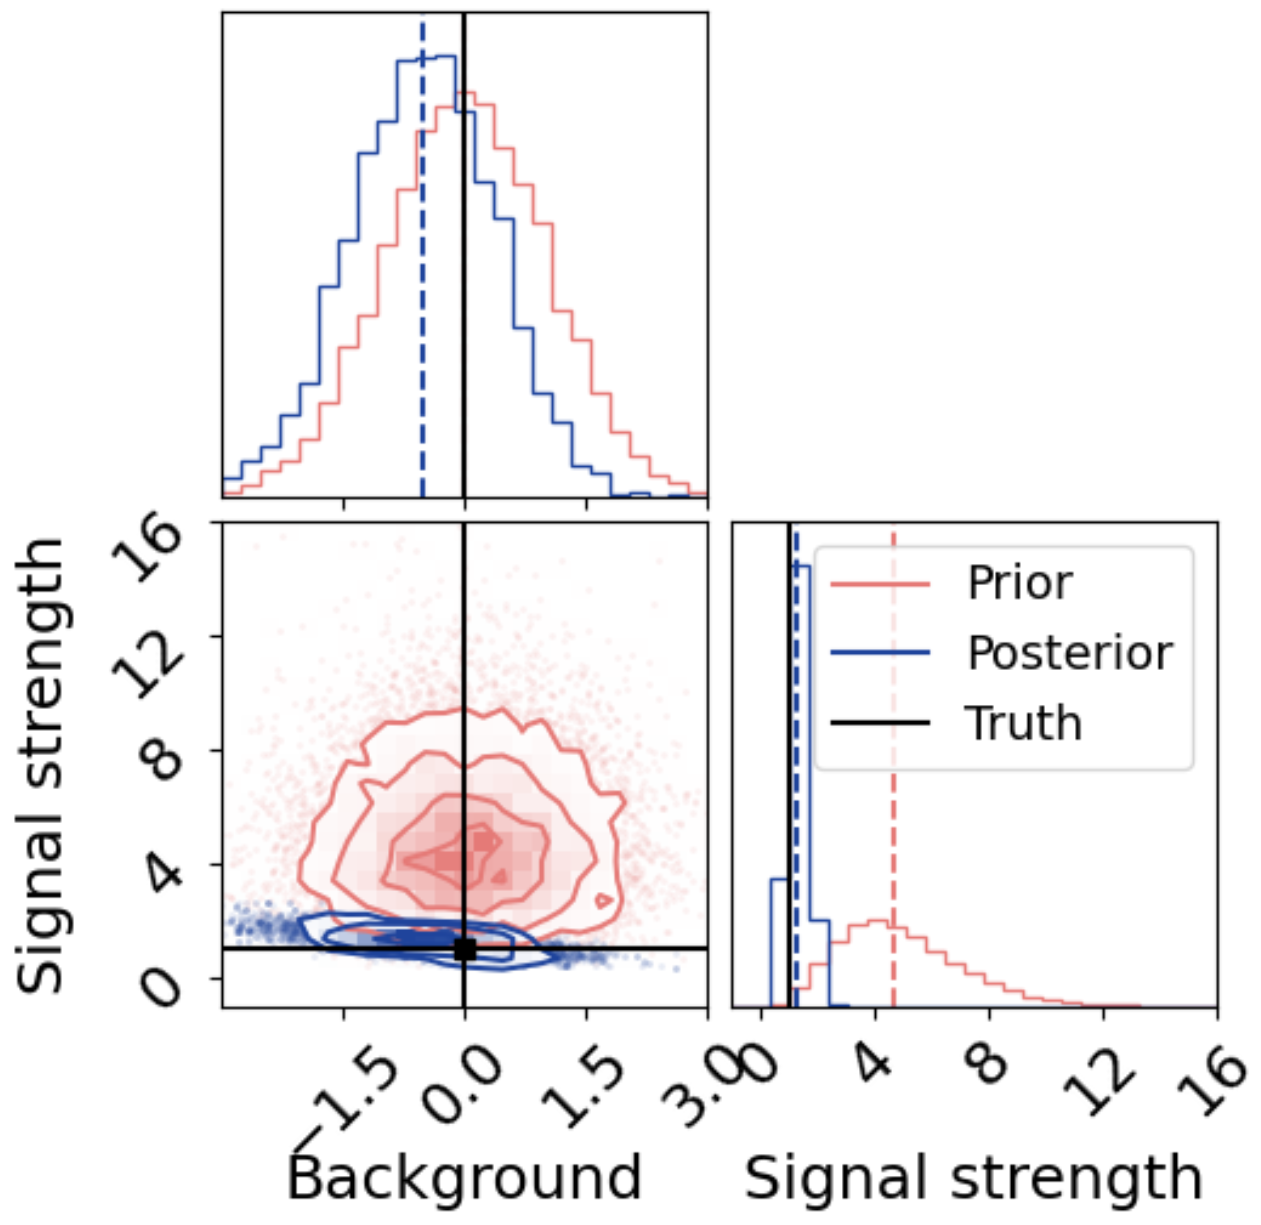
\includegraphics[width=\textwidth]{figures/corner.png}
                 \caption{Correlation for signal and background distribution. Indicated in black is the underlying truth.}
                 \label{corner}
             \end{subfigure}
        \hspace{0.2\textwidth}
             \begin{subfigure}[b]{0.3\textwidth}
                 \centering
                 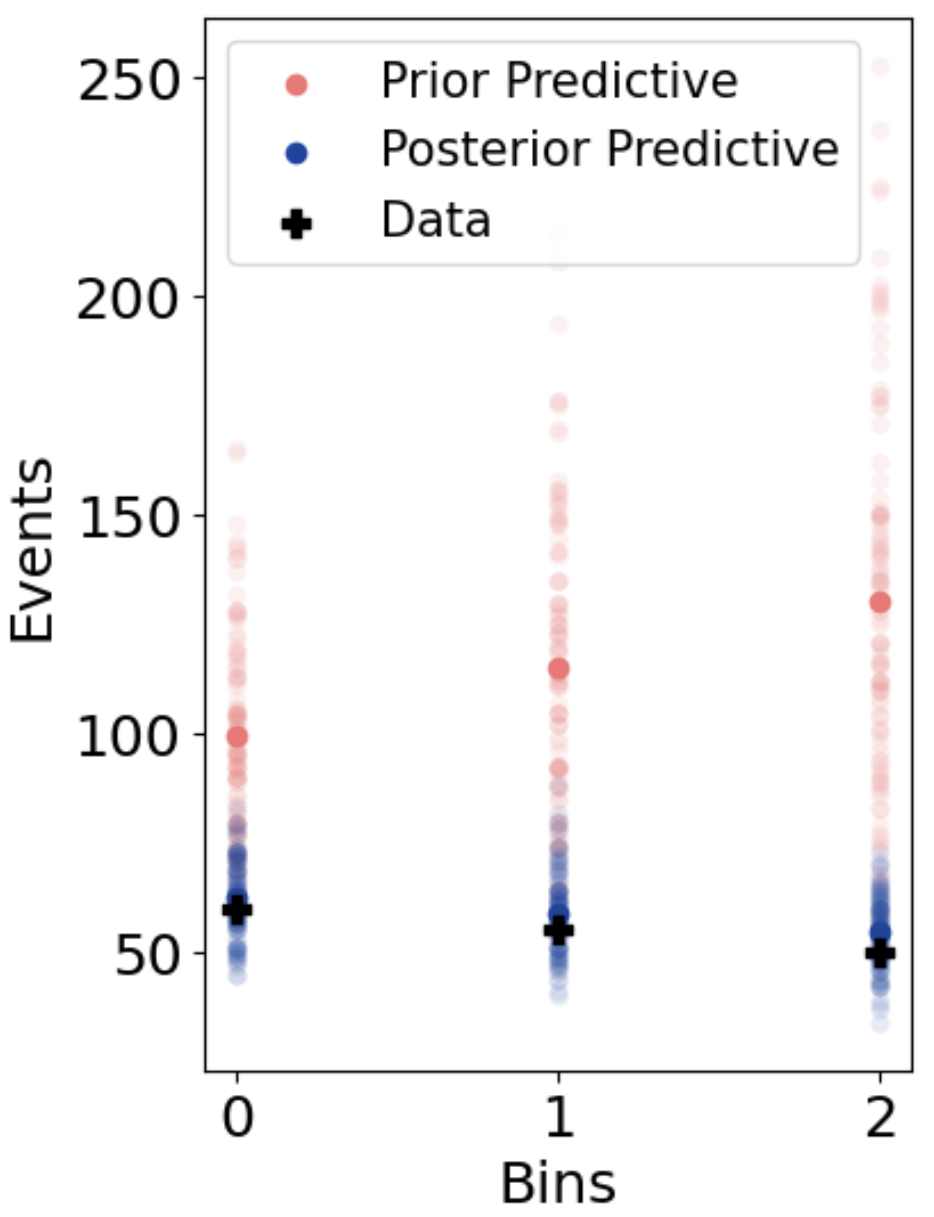
\includegraphics[width=\textwidth]{figures/ppc.png}
                 \caption{Prior and posterior predictive. Indicated in black is the observed data.}
                 \label{ppc}
             \end{subfigure}
        \caption{Comparing prior and posterior distribution for the parameters (\ref{corner}) and predictions for the observations (\ref{ppc}).}
        \label{ppc_corner}
    \end{figure}
\noindent A possible next check is a calibration check, which tests the computational faithfulness of the inference, i.e. whether the distribution of posterior samples can capture a distribution of pseudo-data observations. In particular, if a set of pseudo-observations $x$ is sampled from the prior predictive, the resulting distribution of posteriors should approximate the prior distribution, see Eq.\ref{calibration}.
    \begin{align} \label{calibration}
        p\left(\eta, \chi\right) \overset{!} \approx \int dxd\eta' d\chi' ~  p\left( \eta, \chi | x \right) ~ p\left(y|\eta', \chi'\right)
    \end{align}
\noindent In Fig. \ref{calibrationPlot} this is visualised for the simple model introduced above.
    \begin{figure} %[h]
        \centering
        % \captionsetup{justification=centering}
        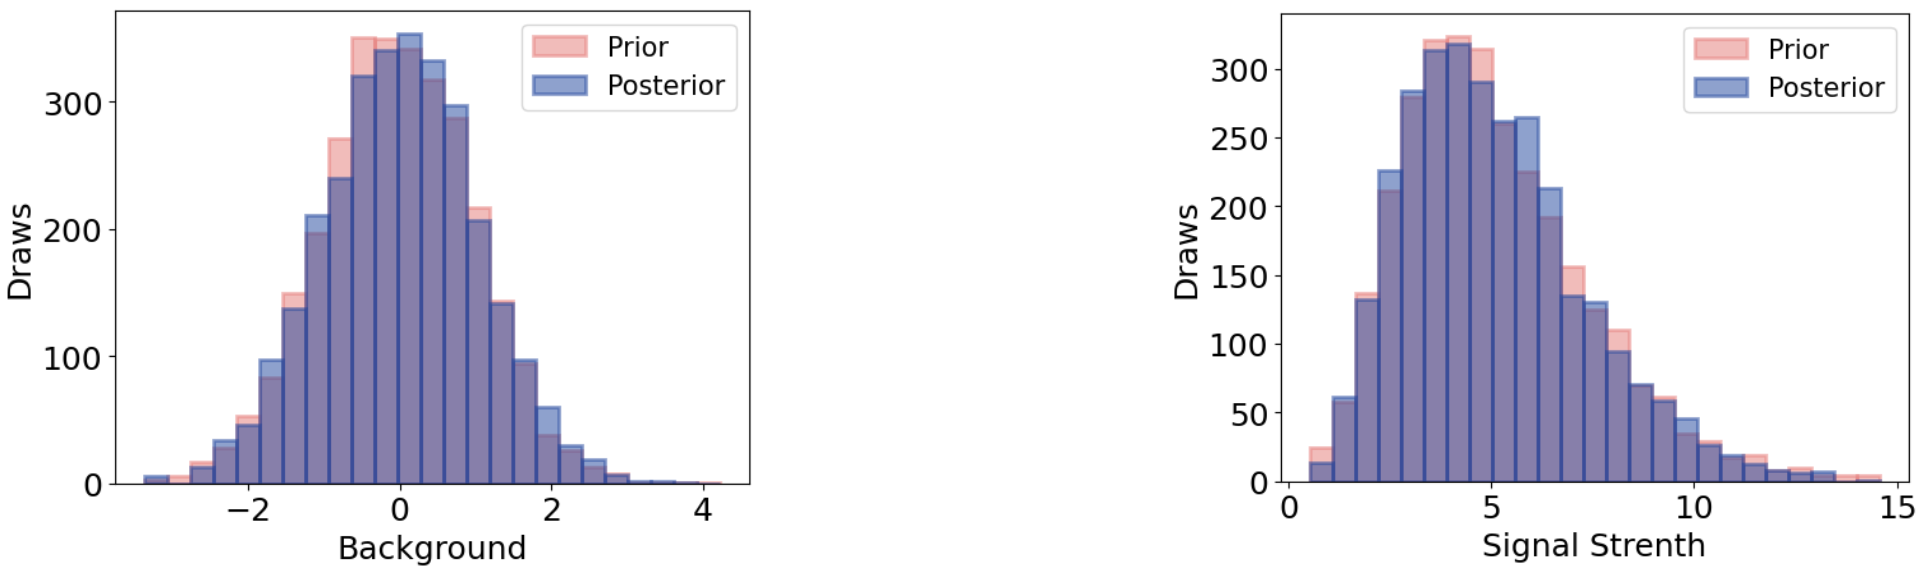
\includegraphics[width=10cm]{figures/calibration.png}
        \centering
        \caption{Calibration check for the signal POI and the background using 3000 pseudo-observations drawn from the prior predictive.}
        \label{calibrationPlot}
    \end{figure}
